\documentclass[11pt, oneside]{article}   	% use "amsart" instead of "article" for AMSLaTeX format
\usepackage{geometry}                		% See geometry.pdf to learn the layout options. There are lots.
\geometry{letterpaper}                   	% ... or a4paper or a5paper or ... 
%\geometry{landscape}                		% Activate for rotated page geometry
\usepackage[parfill]{parskip}    	% Activate to begin paragraphs with an empty line rather than an indent
\usepackage{graphicx}				% Use pdf, png, jpg, or eps§ with pdflatex; use eps in DVI mode
								% TeX will automatically convert eps --> pdf in pdflatex		
\usepackage{amssymb}
\usepackage{amsmath}
\usepackage{hyperref}
\usepackage{makecell} % Add this to your preamble



\title{scPerturb: single cell perturbation}
\author{Sicheng Yi}
\date{05/04/2025}		

\begin{document}
\maketitle


\begin{abstract}
This project investigates how drug perturbations affect gene expression in single cells, with the goal of identifying potential drug candidates for treating leukemia. By modeling the up and down regulation of genes across various peripheral blood mononuclear cell (PBMC) types, including T cells, B cells, NK cells, and myeloid cells, I aim to predict transcriptomic responses to drug compounds. I employ deep learning models, such as multilayer perceptrons (MLPs) and Transformer , to learn from high-dimensional gene expression and molecular features. The results show that these models can more accurately forecast cell-specific differential expression patterns, enabling informed drug screening and prioritization.
\end{abstract}


\section*{Introduction}

Each year, millions of people die from cancer, and acute leukemia remains one of the most prevalent and deadly forms. Understanding how chemical drug compounds influence gene regulation in peripheral blood mononuclear cells (PBMCs) is crucial to developing effective treatments. The experimental setup used to study this biological process is illustrated in Figure~\ref{fig:pbmc}.


\begin{figure}[htbp]
  \centering
  \includegraphics[width=0.8\textwidth]{pbmc.png}
  \caption{Visualization of PBMC data.}
  \label{fig:pbmc}
\end{figure}

In this experiment, blood samples from both healthy individuals and cancer patients are analyzed using single-cell RNA sequencing (scRNA-seq) and chromatin accessibility profiling (scATAC-seq). Over 140,000 individual cells are perturbed with 144 distinct chemical compounds, and their gene expression responses are recorded for more than 18,000 genes. These cells are further categorized into immune subtypes, including CD4+ T cells, CD8+ T cells, natural killer (NK) cells, B cells, and myeloid cells.

As part of the 2023 NeurIPS Kaggle competition, participants were asked to develop models capable of predicting differential gene expression responses based on cell types and small molecule compound features. This presents a challenging high-dimensional regression task due to two main factors: (1) the input features, such as cell type and drug compound, are significantly lower in dimension than the output space of gene expression, and (2) the training and test distributions differ, with training samples primarily from T and NK cells, while test samples consist largely of B and myeloid cells.

This project applies and adapts deep learning methods to this biologically grounded prediction task. By augmenting chemical and cellular input features using domain knowledge (e.g., SMILES-based fingerprinting, categorical encoding), and applying multi-target regression models such as multilayer perceptrons (MLPs) and Transformers, I aim to improve generalization to unseen cell types. Additionally, dimensionality reduction techniques like Principal Component Analysis (PCA) are explored to mitigate the computational challenges posed by extremely high-dimensional gene expression outputs. In addition, I investigate the effectiveness of different architectures and pre-processing strategies on a benchmark single-cell genomics dataset.



\section*{Related Work}

Recent developments in cheminformatics and single-cell perturbation modeling have enabled the application of deep learning to biological response prediction. My work builds on these foundations by combining molecular representations and single-cell transcriptomic.


\textbf{Randomized SMILES} \cite{RandomSmiles}: 

They introduced the idea of randomized SMILES strings, demonstrating that varying atom order in molecular SMILES representations can improve generative model performance. This principle motivates our use of molecular fingerprints and SMILES-derived features to represent chemical perturbations more robustly.

\textbf{scPerturb} \cite{scPerturb}: 

They curated the scPerturb database, which harmonizes 44 single-cell perturbation datasets spanning transcriptomic and proteomics. They propose energy statistics (E-statistics) to quantify perturbation effects across heterogeneous conditions. Their work underscores the need for standardized and scalable evaluation frameworks in perturbation-response modeling.

\textbf{PBMC scRNA-seq} \cite{scRNA-PBMC}:  

They generated a comprehensive single-cell RNA-seq dataset on over 1.3 million PBMCs exposed to various pathogens. Their findings highlight immune cell diversity and context-specific gene regulation, reinforcing the biological motivation for our focus on T, B, NK, and myeloid cells under drug perturbations.

\textbf{scGen} \cite{scGen}:  

They proposed scGen, a deep generative model that uses variational autoencoders to predict cellular responses to perturbations. Their model provides a strong baseline for learning perturbation effects from scRNA-seq data, demonstrating the utility of latent space arithmetic for generalization to unseen conditions.

\textbf{GCN for Drug Effects} \cite{GCNdrug}:

They applied graph convolution networks (GCN) and transfer learning to predict drug-induced gene expression profiles. This approach illustrates the value of encoding chemical structure explicitly through molecular graphs, a direction we may explore in future work.




\section*{Datasets}

This project uses data from the scPerturb NeurIPS 2023 Kaggle Competition, which investigates how drug compounds affect gene expression in peripheral blood mononuclear cells (PBMCs) from both healthy and cancer patients. The dataset includes over 140,000 individual cells categorized into major immune cell types: CD4+ T cells, CD8+ T cells, NK cells, B cells, and Myeloid cells. These cells were exposed to 144 different small-molecule drugs, and differential gene expression was measured across more than 18,000 genes.

The main training dataset, provided as a Parquet file (`de-train.parquet`), contains rows representing unique combinations of cell type and drug compound. The majority of columns correspond to gene names, with each entry denoting the differential expression level induced by the drug. A positive value indicates gene up-regulation, while a negative value indicates down-regulation. The absolute magnitude reflects the strength of the perturbation effect. 

An example of the SMILES string is shown in Table~\ref{tab:de_train}, where all entries for the drug clotrimazole share the same molecular representation. A visual rendering of clotrimazole’s chemical structure is provided in Figure~\ref{fig:smiles}, and its substructure-based encoding is discussed further in the Methods section.



\begin{table}[htbp]
\centering
\small
\begin{tabular}{|l|l|l|l|c|r|r|}
\hline
\textbf{cell\_type} & \textbf{sm\_name} & \textbf{sm\_lincs\_id} & \textbf{SMILES} & \textbf{control} & \textbf{A1BG} \\
\hline
NK cells & Clotrimazole & LSM-5341 & \makecell[l]{Clc1ccccc1C(c1ccccc1)\\(c1ccccc1)n1ccnc1} & False & 0.104720  \\
\hline
T cells CD4+ & Clotrimazole & LSM-5341 & \makecell[l]{Clc1ccccc1C(c1ccccc1)\\(c1ccccc1)n1ccnc1} & False & 0.915953 \\
\hline
T cells CD8+ & Clotrimazole & LSM-5341 & \makecell[l]{Clc1ccccc1C(c1ccccc1)\\(c1ccccc1)n1ccnc1} & False & -0.387721  \\
\hline
T regulatory cells & Clotrimazole & LSM-5341 & \makecell[l]{Clc1ccccc1C(c1ccccc1)\\(c1ccccc1)n1ccnc1} & False & 0.232893  \\
\hline
\end{tabular}
\caption{differential expression level of each genes perturbed by drug among cell types}
\label{tab:de_train}
\end{table}


The distribution of cell types between training and test datasets is notably imbalanced. As shown in Figure~\ref{fig:traintest}, training data predominantly features CD4+/CD8+ T cells and NK cells, while the unseen test data focuses more on B cells and Myeloid cells. This cell-type domain shift presents a significant generalization challenge for predictive models.


\begin{figure}[htbp]
  \centering
  
\includegraphics[width=1.0 \textwidth, height=0.3 \textwidth ]{train-test-split.png}
  \caption{Split of Training Test data}
  \label{fig:traintest}
\end{figure}



\section*{Methods}

\subsection{EDA}

As an initial step, I conducted exploratory data analysis to investigate which genes exhibit strong expression differences between healthy and cancerous conditions. One such gene is \textbf{CD69}, which is known to play a role in immune cell activation and has been previously associated with hematological malignancies.

Figures~\ref{fig:CD69healthy} and~\ref{fig:CD69MPAL} show the expression levels of CD69 in healthy patients and patients with mixed phenotype acute leukemia (MPAL), respectively. In healthy individuals, CD69 expression is relatively low across most immune cell types (Figure~\ref{fig:CD69healthy}). In contrast, MPAL samples show strong overexpression of CD69 in T/NK cells and, notably, in Myeloid cells (Figure~\ref{fig:CD69MPAL}).

These findings suggest that CD69 overexpression may be indicative of leukemic transformation or immune dysregulation in MPAL. Since over 18,000 genes are profiled in this dataset, identifying compounds that can selectively downregulate oncogene-like targets such as CD69 could be of therapeutic interest in blood cancers.

\begin{figure}[htbp]
  \centering
  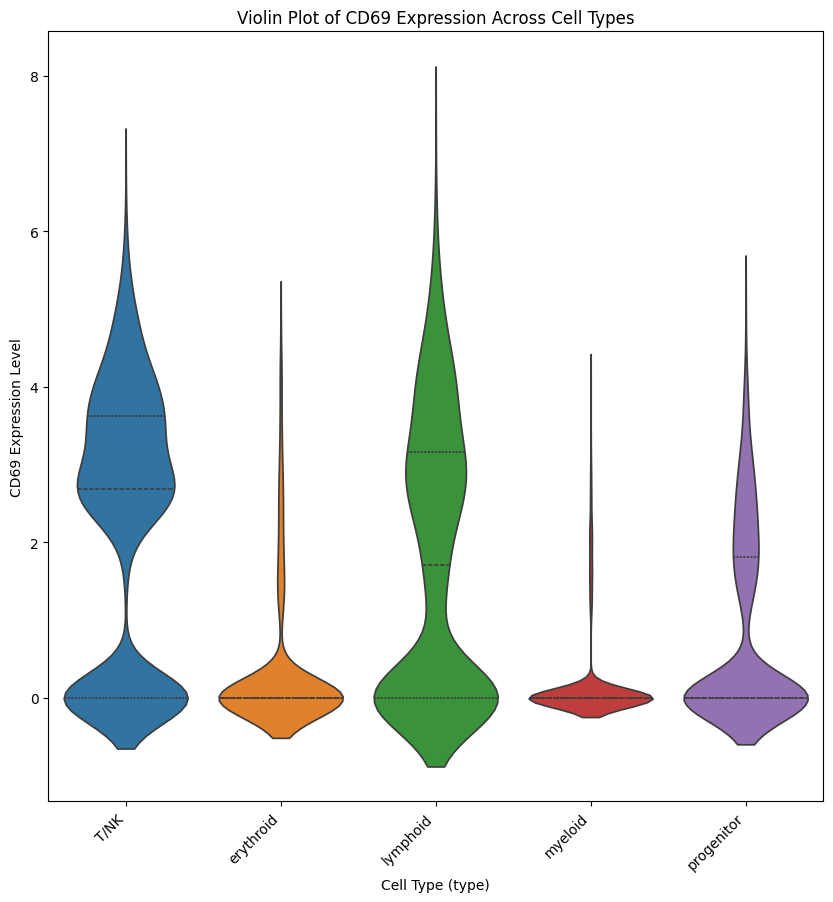
\includegraphics[width=0.3\textwidth]{CD69-health.png}
  \caption{gene CD69 healthy}
  \label{fig:CD69healthy}
\end{figure}


\begin{figure}[htbp]
  \centering
  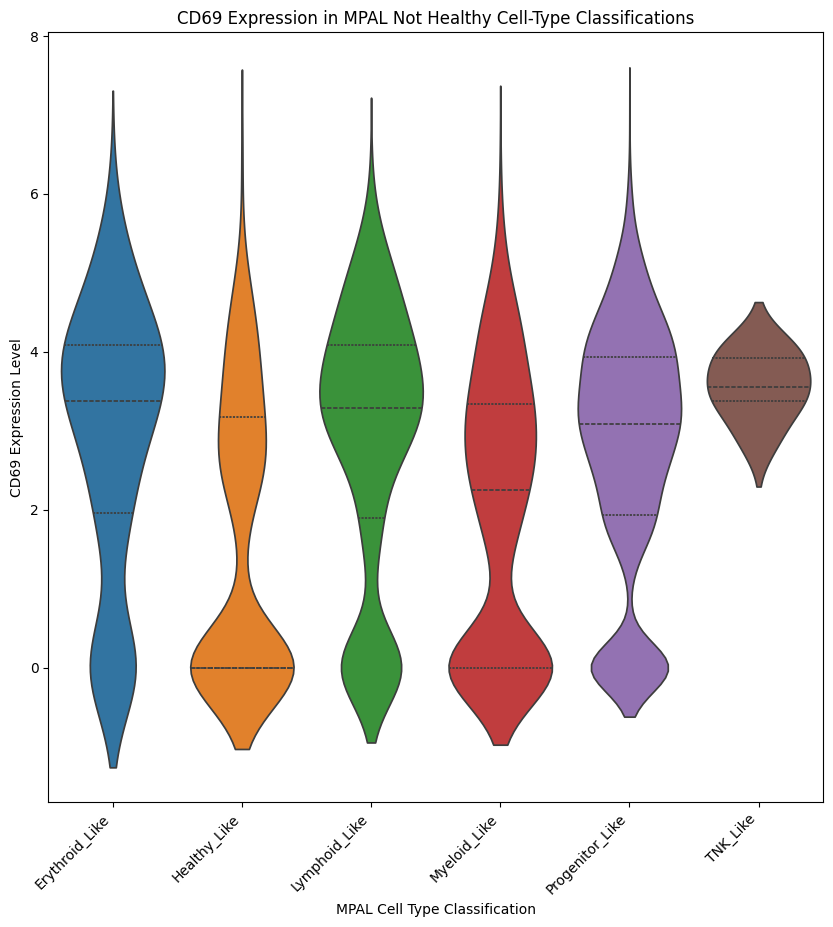
\includegraphics[width=0.3\textwidth]{CD69-MPAL.png}
  \caption{gene CD69 MPAL leukemia}
  \label{fig:CD69MPAL}
\end{figure}


\subsection{Data Augmentation}

One of the major challenges in this project is the disparity between the relatively low-dimensional input space—comprising categorical features such as cell types, small molecule (SM) drug names, SMILES strings, and control status—and the high-dimensional output space, which includes differential gene expression values for over 18,000 genes. To bridge this gap and improve model performance, I implemented several strategies for augmenting the input features.

First, I computed summary statistics—mean, standard deviation, and median—of the gene expression levels grouped by both drug and cell type. These statistical features were added to both training and test data. Incorporating these values provided the model with useful priors and significantly improved baseline performance by offering a general view of how each drug-cell pair behaves.

Second, I enriched the chemical representation of drugs by processing their SMILES (Simplified Molecular-Input Line-Entry System) strings. For instance, the compound clotrimazole, shown in Figure~\ref{fig:smiles}, was decomposed into chemical substructures (Figures~\ref{fig:smiles1} and~\ref{fig:smiles2}). I then built a sparse count matrix to represent the frequency of these substructures across all 144 compounds. This matrix was used as an additional set of features, enabling the model to capture chemical similarities and differences more explicitly.

Third, I employed the \texttt{RDKit} chem informatics toolkit to compute Morgan Finger prints from the SMILES strings. These fingerprints provide a fixed-length numerical encoding that captures the presence and connectivity of molecular substructures. Adding these features allowed the model to learn chemical properties beyond the raw SMILES strings, offering a richer biochemical representation of each drug.

Fourth, since both the cell type and drug compound columns are categorical, I applied standard encoding techniques. One-hot encoding and label encoding were used to transform these categories into numerical formats suitable for input into machine learning models.

Given the large number of additional features introduced—particularly from the sparse substructure count matrix and Morgan Fingerprints—the dimensionality of the input space became very high. To address this and to reduce computational cost, I applied Principal Component Analysis (PCA) to project the augmented input features into a lower-dimensional space while retaining most of the variance. This step not only helped speed up model training but also reduced the risk of overfitting by eliminating noisy and redundant features.



\begin{figure}[htbp]
  \centering
  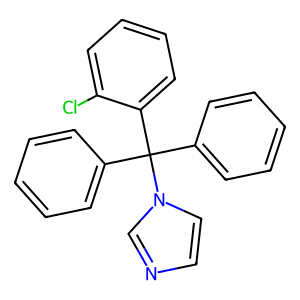
\includegraphics[width=0.3\textwidth]{smiles1.png}
  \caption{Visualization of clotrimazole.}
  \label{fig:smiles}
\end{figure}

\begin{figure}[htbp]
  \centering
  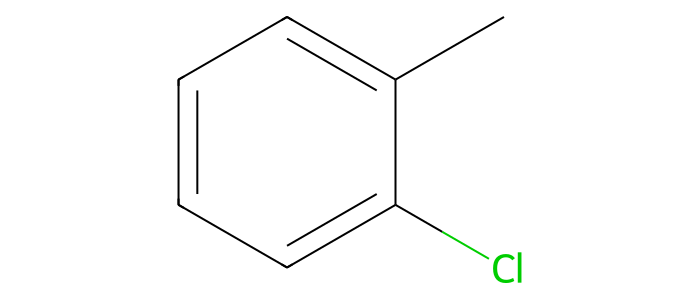
\includegraphics[width=0.3\textwidth]{smiles1-split1.png}
  \caption{clotrimazole sub module 1}
  \label{fig:smiles1}
\end{figure}

\begin{figure}[htbp]
  \centering
  
\includegraphics[width=0.3\textwidth]{smiles1-split2.png}
  \caption{clotrimazole sub module 2}
  \label{fig:smiles2}
\end{figure}



\subsection{Models}

\begin{figure}[htbp]
  \centering
  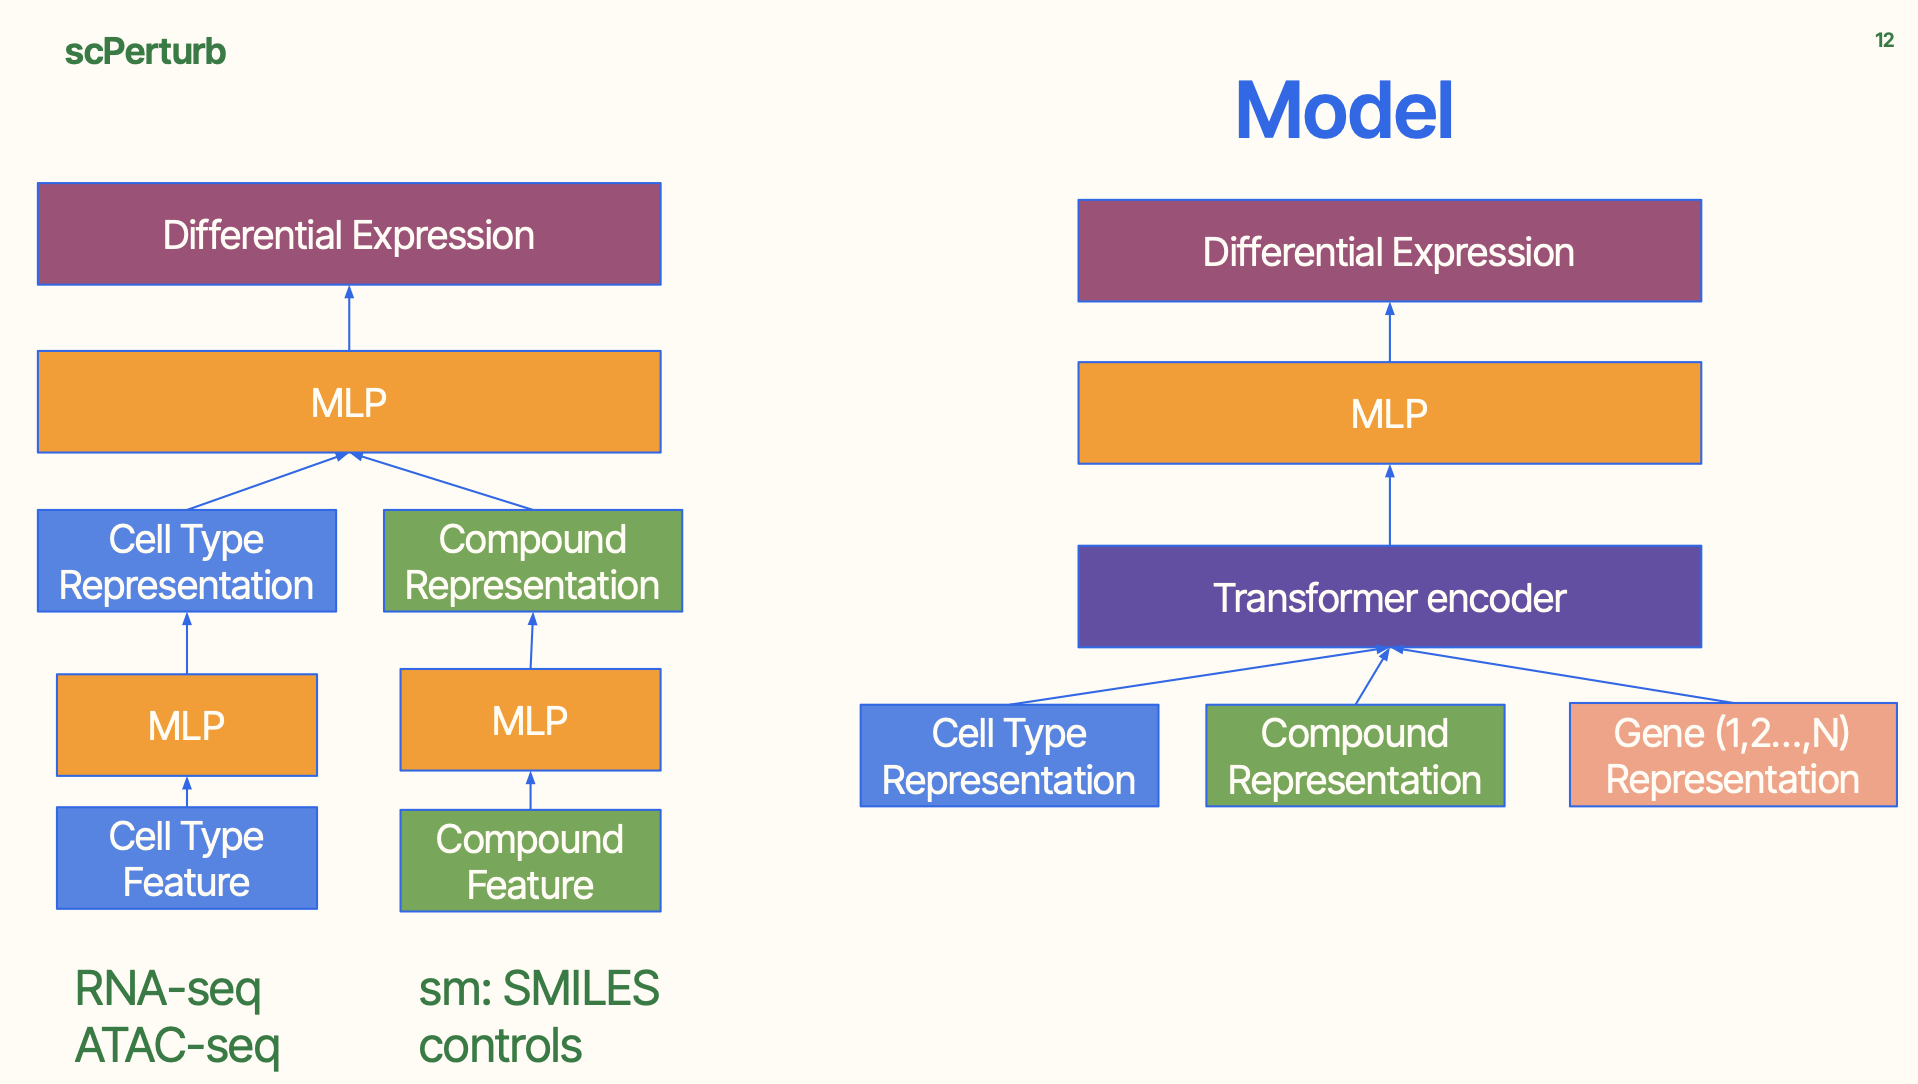
\includegraphics[width=1.0 \textwidth]{models.png}
  \caption{Models}
  \label{fig:models}
\end{figure}


To model the relationship between cell types, drug compounds, and the resulting gene expression profiles, I implemented and compared two deep learning architectures: a Multi-Layer Perceptron (MLP) and a Transformer-based model, as visualized in Figure~\ref{fig:models}.


\paragraph{MLP Architecture:}
The MLP model consists of a deep feedforward network designed to process high-dimensional continuous features. After data augmentation, the input dimension can be as high as 56,000+, so dimensionality reduction using PCA is optionally applied. The architecture includes four fully connected layers with decreasing hidden dimensions: 4096, 2048, 1024, and 512. Each layer is followed by batch normalization, ReLU activation, and dropout to improve generalization. The final output layer maps the 512-dimensional representation to 18,211 gene targets using a linear layer. This model directly learns a mapping from the augmented numerical features—including statistics (mean, std, median), Morgan fingerprints, and SMILES substructure counts—to gene expression profiles.


\paragraph{Transformer-Based Architecture:}
The second model is a TabTransformer-like architecture that separately processes categorical and continuous features. Categorical features, such as cell types and drug compounds, are one-hot encoded and projected into an embedding space using a linear layer. These embeddings are then passed through a Transformer encoder with one layer and eight attention heads to capture interactions between discrete categories. In parallel, the continuous features (e.g., gene statistics, SMILES fingerprints) are normalized and projected into the same embedding dimension using a fully connected branch with Layer Norm, ReLU, and dropout. The embeddings from both categorical and continuous branches are concatenated and passed through a final MLP with hidden size 1024 and dropout before producing the final output of 18,211 gene predictions.

\paragraph{Design Motivation:}
The MLP model leverages the full expressive power of dense connections and is particularly suited to large numerical feature spaces. The Transformer model introduces a more structured inductive bias, allowing it to learn complex interactions among categorical features while still benefiting from continuous inputs. By comparing these two architectures, this project explores how different neural inductive biases affect generalization on a high-dimensional, imbalanced biological prediction task.


\section*{Evaluation}

\begin{figure}[htbp]
  \centering
  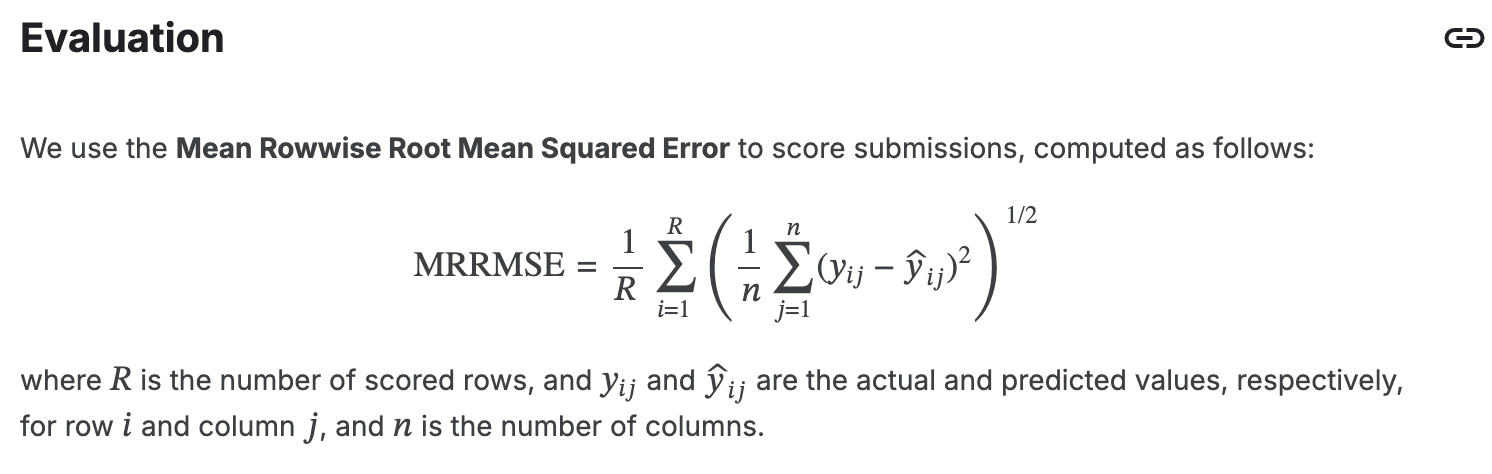
\includegraphics[width=1.0 \textwidth]{loss.png}
  \caption{MRRMSE loss}
  \label{fig:rmse}
\end{figure}

To evaluate model performance, I use a custom variant of the Root Mean Square Error (RMSE), computed at the cell-drug pair level. Specifically, for each sample (i.e., a cell type and drug compound pair), I compute the RMSE across the 18,211 predicted gene expression values and then average this score across all samples. This metric is referred to as the Mean Row-wise RMSE (MRRMSE) and is well-suited to this multi-output regression task, as it treats each row independently and prevents genes with inherently higher variance from dominating the loss. The loss function is shown in Figure~\ref{fig:rmse}. 

\subsection*{Training Setup}

Both MLP and Transformer models are trained using the standard mean squared error (MSE) loss. I split the data into training and validation sets and monitored both training and validation loss over 10 epochs. The models are trained using the Adam optimizer with an initial learning rate of $1 \times 10^{-3}$, and I use a learning rate scheduler (`ReduceLROnPlateau`) to adapt the learning rate based on validation performance. The training loop includes model check pointing, where the model with the lowest validation loss is saved. Figure~\ref{fig:rmse} shows the training and validation loss curves, which help visualize convergence and potential overfitting.

\subsection*{Test Evaluation}

After training, I optionally run the model on a held-out test set and compute the final MSE to assess generalization. 





\section*{Result}

\begin{figure}[htbp]
  \centering
  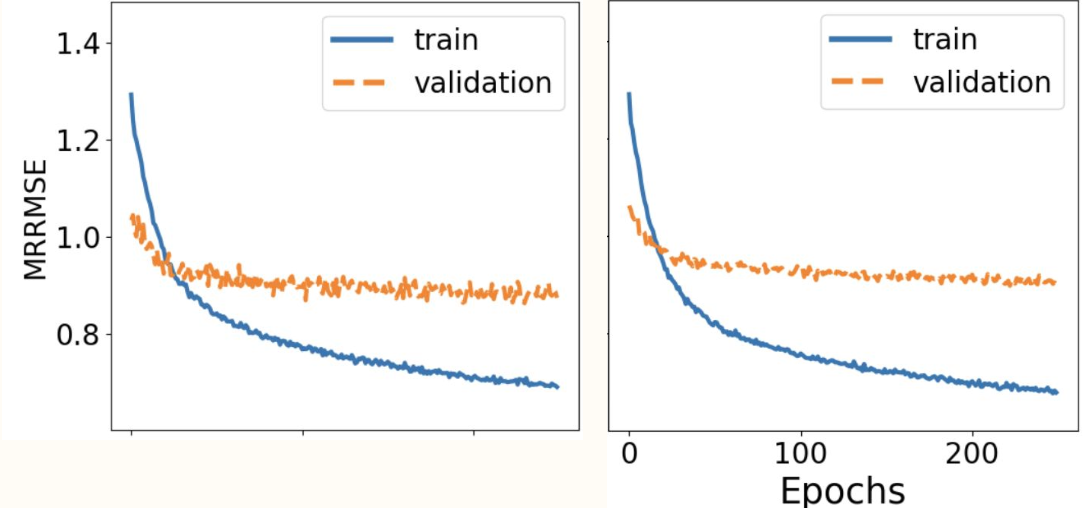
\includegraphics[width=1.0 \textwidth]{training.png}
  \caption{MRRMSE loss}
  \label{fig:training}
\end{figure}


Figure~\ref{fig:training} shows the MRRMSE loss curves for both MLP and Transformer models. The MLP model converges more quickly on the validation set, whereas the Transformer requires slightly more epochs to achieve a comparable level of validation loss. However, both models exhibit signs of overfitting after approximately 100 epochs, as indicated by the divergence between steadily decreasing training loss and plateauing validation loss.


\begin{table}[htbp]
\centering
\begin{tabular}{|l|c|c|}
\hline
\textbf{MRRMSE} & \textbf{MLP} & \textbf{Transformer} \\
\hline
Validation & 0.86 & 0.90 \\
\hline
Test       & 0.93 & 0.87 \\
\hline
\end{tabular}
\caption{MRRMSE scores for MLP and Transformer models on validation and test sets.}
\label{tab:mrrmse_results}
\end{table}


As shown in Table~\ref{tab:mrrmse_results}, while the MLP achieves slightly better performance on the validation set due to faster convergence, it under performs on the hidden test set. In contrast, the Transformer achieves a lower MRRMSE on the test data, suggesting better generalization.

The Transformer model likely benefits from its attention mechanism, which helps capture dependencies between categorical and numerical features. This becomes especially advantageous in the presence of distribution shifts or imbalanced categories—such as the under representation of certain cell types in the training set compared to the test set.

For reference, top-performing models on the Kaggle leader board utilized ensemble techniques combining 4–5 diverse models, achieving MRRMSE scores around 0.75.



\section*{Conclusion}

This project demonstrates that deep learning combined with feature engineering can significantly enhance the prediction of gene expression changes in single cells subjected to chemical perturbations. By augmenting limited categorical inputs with derived numerical features, such as statistical summaries, SMILES-based substructure counts, and molecular fingerprints, I was able to expand the feature space and improve models toward capturing more biologically meaningful patterns.

Between the two models explored, the Transformer demonstrated superior generalization on the unseen test set, particularly in handling distribution shifts across cell types. This suggests that its attention mechanism is better equipped to model complex, high-dimensional relationships inherent in transcriptomic data. In contrast, the MLP model, while converging faster during training, was more prone to overfitting and exhibited higher test error.

Future work could explore ensemble methods to combine the strengths of multiple models, as well as incorporate graph neural networks to better model molecular structures. In addition, semi-supervised learning could help leverage large amounts of unlabeled perturbation data, potentially improving performance and accelerating the discovery of candidate compounds for leukemia treatment.





\section*{Code}

The code for scPerturb is available on Github: 
\href{https://github.com/tigeryi1998/scPerturb}{Github Link}

The 2023 NeurIPS Kaggle Competition:
\href{https://www.kaggle.com/competitions/open-problems-single-cell-perturbations/overview}{Kaggle Link}



\begin{thebibliography}{9}

\bibitem{RandomSmiles}
Arús-Pous, J., Johansson, S.V., Prykhodko, O. et al.
\textit{Randomized SMILES strings improve the quality of molecular generative models. J Cheminform 11, 71 (2019)}. https://doi.org/10.1186/s13321-019-0393-0


\bibitem{scPerturb}
Peidli S et al.
\textit{scPerturb: harmonized single-cell perturbation data. Nature Methods. (2024)}.
https://doi.org/10.1038/s41592-023-02144-y


\bibitem{scRNA-PBMC}
Oelen, R., de Vries, D.H., Brugge, H. et al.
\textit{Single-cell RNA-sequencing of peripheral blood mononuclear cells. Nature Communication 13, 3267 (2022)}.
https://doi.org/10.1038/s41467-022-30893-5

\bibitem{scGen}
Lotfollahi, M., Naghipourfar, M., Theis, F.J.  
\textit{scGen predicts single-cell perturbation responses.}  
Nat Methods 16, 715–721 (2019). 
https://doi.org/10.1038/s41592-019-0494-8

\bibitem{GCNdrug}
Cao, Z., Yuan, F.  
\textit{Predicting drug-induced gene expression profiles using graph convolutional networks and transfer learning.}  
Bioinformatics 37(19), 3245–3252 (2021). https://doi.org/10.1093/bioinformatics/btab264


\end{thebibliography}



\end{document} 